\chapter{Literature Review and Related Works}
\section{Literature Review}
Cyberspace around the world has been the target of distributed - Denial of Service (DDoS) attacks that have evolved into one of the most pressing security threats of the current century \cite{devi2018cyberspace}. DDoS attacks operate by inundating a target system, a network, or an application with traffic originating from a number of IP addresses, all of which are under the attacker’s control, this is called a botnet \cite{poonia2024comprehensive}. Such botnets are made up of the devices with infected malware that conduct actions under a planned order unknown to their owners.
\\
New networked systems, especially the Internet of Things, have increased the risk of DDoS attacks due to the growth of new technologies. Most IoT devices have poor setup security and are easily compromised for use in large-scale botnet systems including the Mirai. This botnet exposed the frightening impact of DDoS attacks by ‘offline’ several key DNS providers that make the Internet unreachable \cite{joodat2017distributed}.
\\
\begin{figure}[h]
    \centering
    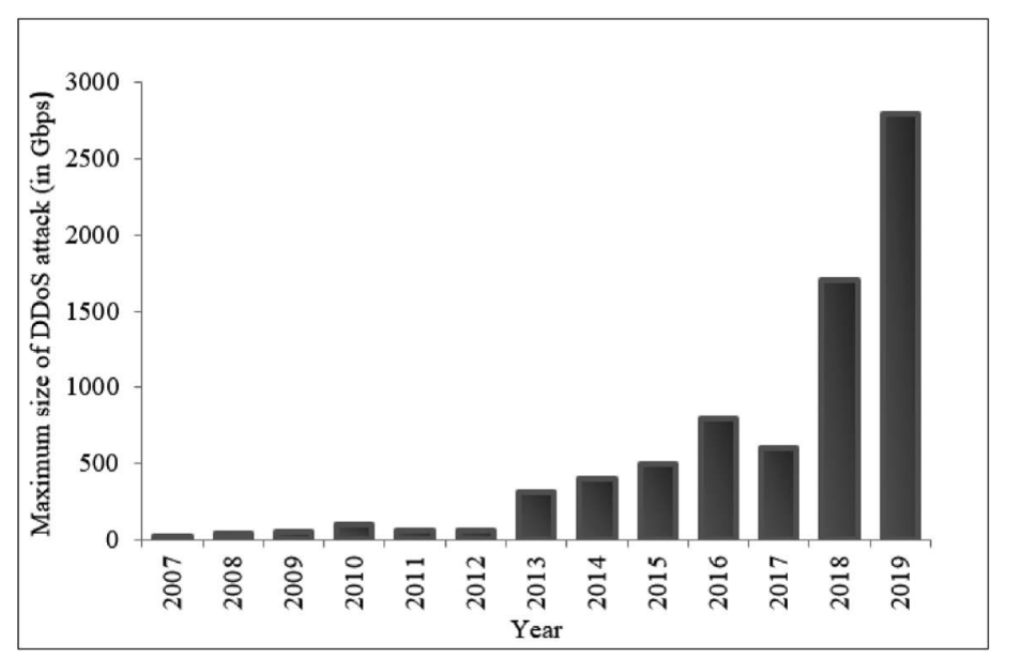
\includegraphics[width=0.8\linewidth]{thesis/DDoSGraph.png}
    \caption{The largest DDoS record each year}
    \label{fig:enter-label}
\end{figure}
\\
\\
DDoS attacks can be classified into two types based on their methods: direct and reflected. Direct attacks require attackers to interact directly with the target host. They are often combined with network-layer attacks to flood the victim with a large number of packets. Reflected attacks involve intermediate servers, where attackers send a large number of packets to the intermediate server by spoofing the source IP address as the target host. The intermediate server then returns a large number of packets to the target host \cite{gai2024introduction}. Examples of such attacks include DNS reflection attacks and SSDP reflection attacks \cite{arukonda2015innocent}. Because the ratio of response packets to request packets is much greater than 1, these attacks are also known as DDoS amplification attacks \cite{sieklik2016evaluation}. 
\\ 
By classifying DDoS attacks based on their objectives and methods, they can be divided into four types: 
\begin{enumerate}
    \item Network-layer attacks: The network layer is charged with the role of taking the traffic off the transport layer and get ready to cross over to data link layer that brings about the accomplishment of end-to-end delivery of packets between the nodes \cite{g2016network}. This attack can be applied in a number of ways so as to render the system useless. It is not used to steal or modify the information but to attack the system availability and make it unavailable. A huge quantity of radiofrequency signals that could be transmitted by a particular system could interfere with and halt the functioning of all sensor nodes, thereby, causing a DDoS attack \cite{ahmed2021networking}. Examples include TCP SYN flood and UDP flood attacks.
    \item Application-layer attacks: The attacks do not require a large volume of attack to be launched as compared to the network layer attacks. They also employ valid application layer requests thus rendering current defense mechanisms hard to identify them. They are used to target a large range of resources at the application layer and can take a server out much quicker and, more importantly, with much more stealth than any network layer DDoS attack \cite{praseed2018ddos}. These attacks exploit the application-layer protocols in order to get as much processing power in the victim’s server as possible. The types include HTTP slow attacks and CC attacks \cite{shema2010seven}. 
    \item Direct attacks: The attack packets are directly sent to the target host. Target responds to the source address of that packet but majority of the responses are not passed to zombies since majority of the packets use spoofed source IP address to ensure that zombies conceal themselves \cite{park2014computer}. The direct DDoS attack is launched by sending numerous SYN request packets towards victim server \cite{pan2005parallel}. Most of the are used in conjunction with the network layer attacks in an effort to deluge the victim with many packets.
    \item Reflected attacks: By reflecting their flooding traffic off of reflectors; i.e., by spoofing requests to the victim to a large pool of Internet servers which will then each send their respective replies to the victim, attackers can make such distributed denial-of-service attacks more challenging to defend against. The flood caused by this dilution of locality in the flooding stream makes it difficult for the victim to (a) isolate the attack traffic so as to block it, and (b) traceback techniques to identify the source of streams of packets with spoofed source addresses \cite{paxson2001analysis}. Owing to source IP address spoofing, the attackers make the packets originate from the victim host, and they flood the intermediate server with packets. An intermediate server will on the other hand sends a large number of packets back to the victim host thus increasing the traffic of the attack. Some are namely DNS reflection attacks and SSDP reflection attacks.
\end{enumerate}
\section{Related Works}
Since this is a classical topic, there are many projects and research on DDoS attacks to look into. However, not every information is needed in this thesis. This section aims at giving an extensive summary of available studies and real world applications, which will be used in the process of simulating Distributed Denial of Service (DDoS) attacks and the placement of intrusion detection and prevention systems (IDS/IPS). This report discusses the evolution and features of different DDoS attack methods, how network simulation software, specifically GNS3, can be used in cybersecurity research, and how IDS/IPS systems like Suricata  can be used to identify and respond to such threats. This section serves to detect the existing trends, techniques and limitations in the area via analyzing previous researches and projects, thus creating a background to the present research and defining the importance of the given project in continuing the already existing efforts in experimentation and education in the area of network security. 
\\ 
The author, Stallings, explains that the application of IoT devices has amplified the challenge of DDoS many times to the attackers. He also calls for a proper grasp of the requisite modern structures of the network to prevent such attack. For instances, the book gives an illustration of how unsecure IoT devices are and how they can be used to create botnets which are used in executing high traffic attack such as Mirai botnet. Stallings, W. (2017). Foundations of Modern Networking: SDN, NFV, QoE, IoT and Cloud are indispensable recent trends which are being widely studied and implemented.
Stallings goes further by stating that the rise of IoT based devices have made DDoS a lot more easier to execute. For this kind of attacks, he focuses on the architecture and weakness of today’s networks to counter act. For example, the book describes how devices that lack sufficient security can be used to create botnets for massive attack such as the Mirai botnet as highlighted in the book \cite{stallings2015foundations}.
\\
Distributed Denial of Service (DDoS) attacks have evolved significantly since their emergence in the late 1990s. Initially, attackers used simple flooding techniques such as SYN floods, ICMP floods, and UDP floods to exhaust network bandwidth or server resources. These early attacks often originated from a single machine and were relatively easy to mitigate \cite{da2018detection}. By the early 2000s, attackers began using botnets—networks of compromised computers—to launch large-scale, distributed attacks. Tools like Trinoo, TFN, and LOIC enabled more complex and powerful DDoS operations. The use of application-layer attacks, such as HTTP floods, soon followed, targeting web services more precisely and stealthily \cite{ozccelik2020distributed}. In the 2010s, the rise of the Internet of Things (IoT) brought a new wave of DDoS threats. The Mirai botnet in 2016 marked a significant turning point, as it exploited poorly secured IoT devices to launch record-breaking attacks, some exceeding 1 Tbps \cite{https://web.archive.org}.
\\
Modern DDoS attacks are often multi-vector, combining volumetric, protocol, and application-layer techniques. They may also use reflection and amplification methods (e.g., DNS or NTP amplification) to maximize impact \cite{nikolskaya2017review}. Today, attackers leverage automation, encrypted traffic, and even AI-driven tools, making DDoS defense increasingly complex. IoT networks are highly susceptible to botnet formation, given the often minimal or absent security configurations \cite{long2001trends}. This highlights the importance of securing the firmware of the device and implementing network segmentation to prevent large-scale DDoS attacks. Another book was used during this project to understand more about GNS3 and to demonstrate that it is capable of handling multiple cisco devices and simulate many network scenarios \cite{welsh2013gns3}, which contributes to the development of this project.
\\
Additionally, this project could not be whole without hping3, which is a packet generation tool that allows to create packets, spoof packets and set any number of options desired. We are able to SYN attack, flood the network, IP address spoofing. much functionality to test firewall connectivity, IDS or IPS systems, including Suricata. Also to train Wireshark to create certain type of packet \cite{miller2022cissp}. This project applies hping3 to launch a simulation of DDoS attack on a Linux host. The attack scripts are kept simple and based on National Centre for Communication Security's (NCCS) document \cite{nccs}. Another tool we use for this project is Suricata, an open-source network intrusion detection and prevention system (IDS/IPS). It is expected to observe the traffic on the network and identify various threats, such as malware, intrusion attempts, network anomalies \cite{fadhilah2020performance}. Suricata is written in a rule-based language and is used to inspect network packets in real time, enabling it to detect and take action against suspicious or malicious activity. It can be implemented in form of Intrusion Detection System (IDS) or Intrusion Prevention System (IPS) \cite{gupta2024security}. According to the research called "Suricata-Based Intrusion Detection and Isolation System for Local Area Networks" \cite{sree2024suricata}, we can have an idea how Suricata can be implemented to GNS3 and use such method to capture our data in this project.
\section{Attack Classification}
There are various types of DDoS attacks, each of which has its own effect on multiple levels and would incur damages on distinct areas of a stack. In case with this project, it is reduced to volumetric attacks specifically UDP Flooding. In this form of DDoS attack, a large amount of UDP packets is directed at random ports in the target \cite{g2016network1}. Victim server wastes resources searching on listening of applications on those ports and when it finds none, it will respond through ICMP Destination Unreachable responses \cite{inproceedings}. Such packets flood the bandwidth, and the processing power which results in unavailability or degradation to these services \cite{JAVANMARDI2024103778}.
\subsection{Attack Method in the Project}
\begin{enumerate}
    \item Command Execution
    \\ The attacker machine sends a script (start\_attack.sh) to botnet machines.
    \item Packet Generation
    \\ Each bot runs an hping3 command that initiates a UDP flood toward the victim IP (192.168.56.101).
    \item Packets Flow
    \\ Packets traverse the simulated network using GNS-3's routers and switches, reaching the target.
    \item Detection and Mitigation
    \\ Suricata operates in IPS mode on the victim, inspects incoming traffic and, based on rule thresholds, drops malicious packets and logs alerts.
\end{enumerate}
\begin{figure}[!htb]
    \centering
    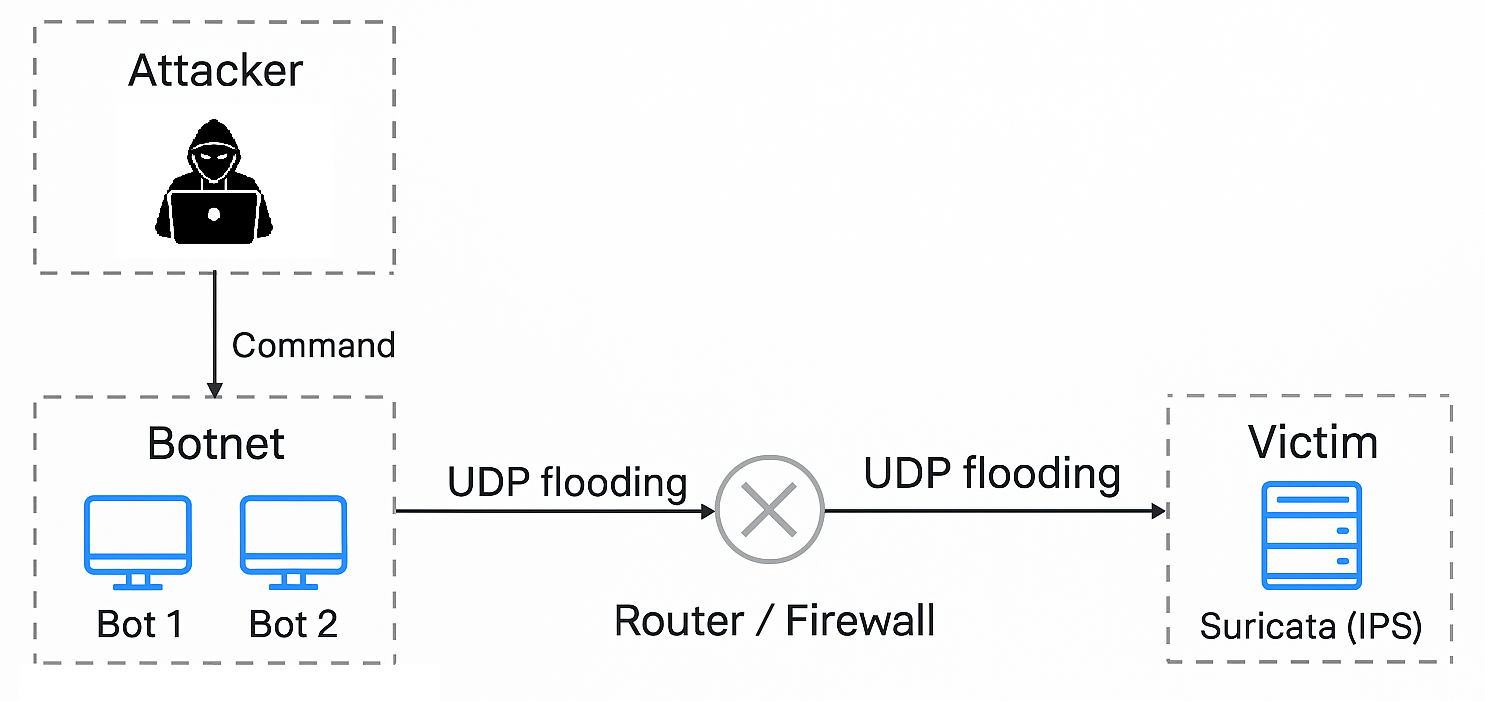
\includegraphics[width=0.8\linewidth]{thesis/attackDiagram.png}
    \caption{Diagram of attack flow}
    \label{fig:enter-label}
\end{figure}
\section{Why UDP Is Used}
This simulation has chosen UDP flooding because of its simplicity and the efficiency of draining the resources, the statelessness of the protocol generates it considerably easier to produce and filter, and its simplicity and its presence in the captures of the packet (no encryption, no handshake).
\begin{table}[!htb]
    \centering
    \begin{tabular}{|c|c|m{5cm}|m{3cm}|}
    \hline
        Attack Type & Target Layer & How it works & Why it is used\\
    \hline
        UDP Flood & Transport & Sends a large number of UDP packets to target ports & Simple to launch.Hard to trace\\
    \hline
       TCP SYN Flood & Transport & Starts many fake TCP connections & Exploits TCP handshake \\
    \hline
        ICMP Flood & Network & Overloads the target with ICMP (ping) requests & Easy but less effective on modern networks\\
    \hline
        DNS Amplification & Application & Tricks DNS servers to send huge replies to the victim & Very powerful with fewer resources needed \\
    \hline
    \end{tabular}
    \caption{Comparison of Common DDoS Attack Types}
    \label{tab:my_label}
\end{table}